\exerciseset{In Exercises}{, sketch $\vec u$, $\vec v$, $\vec u+\vec v$ and $\vec u-\vec v$ on the same axes.}{

\exercise{\mbox{}\\[-2\baselineskip]\begin{minipage}[m]{\linewidth}
\centering
\begin{tikzpicture}[>=stealth]
\begin{axis}[width=1.16\marginparwidth,tick label style={font=\scriptsize},
axis y line=middle,axis x line=middle,name=myplot,axis on top,
xtick=\empty,ytick=\empty,ymin=-4.5,ymax=4.5,xmin=-4.5,xmax=4.5]
\draw [->,thick,draw={\colorone}] (axis cs:0,0) -- (axis cs: 3,1) node [above,black] {\scriptsize $\vec u$};
\draw [->,thick,draw={\colorone}] (axis cs:0,0) -- (axis cs: -1,-4)node [black, left] {\scriptsize $\vec v$};
\end{axis}
\node [right] at (myplot.right of origin) {\scriptsize $x$};
\node [above] at (myplot.above origin) {\scriptsize $y$};
\end{tikzpicture}
\end{minipage}}{\mbox{}\\[-\baselineskip]\begin{minipage}[m]{\linewidth}
\centering
\begin{tikzpicture}[>=stealth]
\begin{axis}[width=1.16\marginparwidth,tick label style={font=\scriptsize},
axis y line=middle,axis x line=middle,name=myplot,axis on top,
xtick=\empty,ytick=\empty,ymin=-4.5,ymax=4.5,xmin=-4.5,xmax=4.5]
\draw [->,thick,draw={\colorone}] (axis cs:0,0) -- (axis cs: 3,1) node [above,black] {\scriptsize $\vec u$};
\draw [->,thick,draw={\colorone}] (axis cs:0,0) -- (axis cs: -1,-4)node [black, left] {\scriptsize $\vec v$};
\draw [->,thick,draw={\colorone}] (axis cs:0,0) -- (axis cs: 2,-3)node [black,below right] {\scriptsize $\vec u+\vec v$};
\draw [->,thick,draw={\colorone}] (axis cs:-1,-4) -- (axis cs: 3,1)node [black,below,pos=.3,sloped] {\scriptsize $\vec u-\vec v$};
\end{axis}
\node [right] at (myplot.right of origin) {\scriptsize $x$};
\node [above] at (myplot.above origin) {\scriptsize $y$};
\end{tikzpicture}
\end{minipage}}

\exercise{\mbox{}\\[-2\baselineskip]\begin{minipage}[m]{\linewidth}
\centering
\begin{tikzpicture}[>=stealth]
\begin{axis}[width=1.16\marginparwidth,tick label style={font=\scriptsize},
axis y line=middle,axis x line=middle,name=myplot,axis on top,
xtick=\empty,ytick=\empty,ymin=-4.5,ymax=4.5,xmin=-4.5,xmax=4.5]
\draw [->,thick,draw={\colorone}] (axis cs:0,0) -- (axis cs: 3,3) node [above,black] {\scriptsize $\vec u$};
\draw [->,thick,draw={\colorone}] (axis cs:0,0) -- (axis cs: -1,-1)node [black, below] {\scriptsize $\vec v$};
\end{axis}
\node [right] at (myplot.right of origin) {\scriptsize $x$};
\node [above] at (myplot.above origin) {\scriptsize $y$};
\end{tikzpicture}
\end{minipage}}{\mbox{}\\[-\baselineskip]\begin{minipage}[m]{\linewidth}
\centering
\begin{tikzpicture}[>=stealth]
\begin{axis}[width=1.16\marginparwidth,tick label style={font=\scriptsize},
axis y line=middle,axis x line=middle,name=myplot,axis on top,
xtick=\empty,ytick=\empty,ymin=-4.5,ymax=4.5,xmin=-4.5,xmax=4.5]
\draw [->,thick,draw={\colorone}] (axis cs:0,0) -- (axis cs: 3,3) node [above,black] {\scriptsize $\vec u$};
\draw [->,thick,draw={\colorone}] (axis cs:0,0) -- (axis cs: -1,-1)node [black, left] {\scriptsize $\vec v$};
\draw [->,thick,draw={\colorone}] (axis cs:0,0) -- (axis cs: 2,2)node [black,above left] {\scriptsize $\vec u+\vec v$};
\draw [->,thick,draw={\colorone}] (axis cs:-1,-2) -- (axis cs: 3,2)node [black,below,pos=.3,sloped] {\scriptsize $\vec u-\vec v$};
\end{axis}
\node [right] at (myplot.right of origin) {\scriptsize $x$};
\node [above] at (myplot.above origin) {\scriptsize $y$};
\end{tikzpicture}

Sketch of $\vec u-\vec v$ shifted for clarity.
\end{minipage}}

% todo convert 11.2#14,15 to asymptote figures
\exercise{\mbox{}\\[-2\baselineskip]\begin{minipage}[m]{\linewidth}
\centering
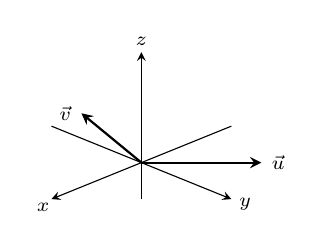
\begin{tikzpicture}[>=stealth]
\begin{axis}[width=175pt,tick label style={font=\scriptsize},axis on top,
axis lines=center,view={135}{35},name=myplot,
xtick=\empty,ytick=\empty,ztick=\empty,
ymin=-1.5,ymax=1.5,xmin=-1.5,xmax=1.5,zmin=-0.5, zmax=1.5,
every axis x label/.style={at={(axis cs:\pgfkeysvalueof{/pgfplots/xmax},0,0)},xshift=-3pt,yshift=-3pt},
xlabel={\scriptsize $x$},
every axis y label/.style={at={(axis cs:0,\pgfkeysvalueof{/pgfplots/ymax},0)},xshift=5pt,yshift=-2pt},
ylabel={\scriptsize $y$},
every axis z label/.style={at={(axis cs:0,0,\pgfkeysvalueof{/pgfplots/zmax})},xshift=0pt,yshift=4pt},
zlabel={\scriptsize $z$}]
\draw [thick,->,draw={\colorone}] (axis cs:0,0,0) -- (axis cs:-1,1,0) node [black,right] {\scriptsize $\vec u$};
\draw [thick,->,draw={\colorone}] (axis cs:0,0,0) -- (axis cs:1,0,1) node [black,left] {\scriptsize $\vec v$};
\end{axis}
\end{tikzpicture}
\end{minipage}}{\mbox{}\\[-\baselineskip]\begin{minipage}[m]{\linewidth}
\centering
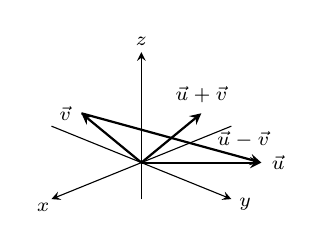
\begin{tikzpicture}[>=stealth]
\begin{axis}[width=175pt,tick label style={font=\scriptsize},axis on top,
axis lines=center,view={135}{35},name=myplot,
xtick=\empty,ytick=\empty,ztick=\empty,
ymin=-1.5,ymax=1.5,xmin=-1.5,xmax=1.5,zmin=-0.5, zmax=1.5,
every axis x label/.style={at={(axis cs:\pgfkeysvalueof{/pgfplots/xmax},0,0)},xshift=-3pt,yshift=-3pt},
xlabel={\scriptsize $x$},
every axis y label/.style={at={(axis cs:0,\pgfkeysvalueof{/pgfplots/ymax},0)},xshift=5pt,yshift=-2pt},
ylabel={\scriptsize $y$},
every axis z label/.style={at={(axis cs:0,0,\pgfkeysvalueof{/pgfplots/zmax})},xshift=0pt,yshift=4pt},
zlabel={\scriptsize $z$}]
\draw [thick,->,draw={\colorone}] (axis cs:0,0,0) -- (axis cs:-1,1,0) node [black,right] {\scriptsize $\vec u$};
\draw [thick,->,draw={\colorone}] (axis cs:0,0,0) -- (axis cs:1,0,1) node [black,left] {\scriptsize $\vec v$};
\draw [thick,->,draw={\colorone}] (axis cs:0,0,0) -- (axis cs:0,1,1) node [black,above] {\scriptsize $\vec u+\vec v$};
\draw [thick,->,draw={\colorone}] (axis cs:1,0,1) -- (axis cs:-1,1,0) node [black,above,pos=.9] {\scriptsize $\vec u-\vec v$};
\end{axis}
\end{tikzpicture}
\end{minipage}}

\exercise{\mbox{}\\[-2\baselineskip]\begin{minipage}[m]{\linewidth}
\centering
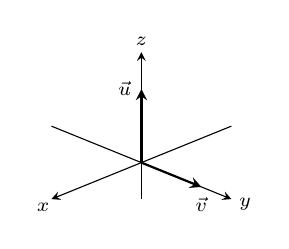
\begin{tikzpicture}[>=stealth]
\begin{axis}[width=175pt,tick label style={font=\scriptsize},axis on top,
axis lines=center,view={135}{35},name=myplot,
xtick=\empty,ytick=\empty,ztick=\empty,
ymin=-1.5,ymax=1.5,xmin=-1.5,xmax=1.5,zmin=-0.5, zmax=1.5,
every axis x label/.style={at={(axis cs:\pgfkeysvalueof{/pgfplots/xmax},0,0)},xshift=-3pt,yshift=-3pt},
xlabel={\scriptsize $x$},
every axis y label/.style={at={(axis cs:0,\pgfkeysvalueof{/pgfplots/ymax},0)},xshift=5pt,yshift=-2pt},
ylabel={\scriptsize $y$},
every axis z label/.style={at={(axis cs:0,0,\pgfkeysvalueof{/pgfplots/zmax})},xshift=0pt,yshift=4pt},
zlabel={\scriptsize $z$}]
\draw [thick,->,draw={\colorone}] (axis cs:0,0,0) -- (axis cs:0,0,1) node [black,left] {\scriptsize $\vec u$};
\draw [thick,->,draw={\colorone}] (axis cs:0,0,0) -- (axis cs:0,1,0) node [black,below] {\scriptsize $\vec v$};
\end{axis}
\end{tikzpicture}
\end{minipage}}{\mbox{}\\[-\baselineskip]\begin{minipage}[m]{\linewidth}
\centering
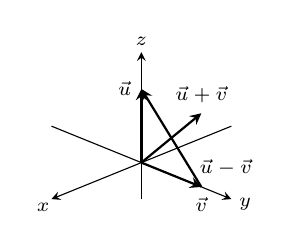
\begin{tikzpicture}[>=stealth]
\begin{axis}[width=175pt,tick label style={font=\scriptsize},axis on top,
axis lines=center,view={135}{35},name=myplot,
xtick=\empty,ytick=\empty,ztick=\empty,
ymin=-1.5,ymax=1.5,xmin=-1.5,xmax=1.5,zmin=-0.5, zmax=1.5,
every axis x label/.style={at={(axis cs:\pgfkeysvalueof{/pgfplots/xmax},0,0)},xshift=-3pt,yshift=-3pt},
xlabel={\scriptsize $x$},
every axis y label/.style={at={(axis cs:0,\pgfkeysvalueof{/pgfplots/ymax},0)},xshift=5pt,yshift=-2pt},
ylabel={\scriptsize $y$},
every axis z label/.style={at={(axis cs:0,0,\pgfkeysvalueof{/pgfplots/zmax})},xshift=0pt,yshift=4pt},
zlabel={\scriptsize $z$}]
\draw [thick,->,draw={\colorone}] (axis cs:0,0,0) -- (axis cs:0,0,1) node [black,left] {\scriptsize $\vec u$};
\draw [thick,->,draw={\colorone}] (axis cs:0,0,0) -- (axis cs:0,1,0) node [black,below] {\scriptsize $\vec v$};
\draw [thick,->,draw={\colorone}] (axis cs:0,0,0) -- (axis cs:0,1,1) node [black,above] {\scriptsize $\vec u+\vec v$};
\draw [thick,->,draw={\colorone}] (axis cs:0,1,0) -- (axis cs:0,0,1) node [black,right,pos=.2] {\scriptsize $\vec u-\vec v$};
\end{axis}
\end{tikzpicture}
\end{minipage}}

}
